\documentclass{book}
\usepackage[paperwidth=3.5in, paperheight=4.75in, margin=0.15in]{geometry}
%\usepackage[margin=1in,footskip=0.25in]{geometry}
\usepackage{fancyvrb}
\usepackage{url}
\usepackage{graphicx}

%opening
\title{}
\author{}

\begin{document}

\maketitle
\chapter{REVISION}
\section{CHANGES}
\begin{tabular}{| l | c | r |}
\hline
Version & Description of change & Date \\ \hline
0.1 & First Draft & 2014/08/25\\
\hline
\end{tabular}

\chapter{IMPORTANT INITIALIZATION}
 

\chapter{Analog to Digital Convertor}
\section{USER SPACE ACCESS}
The ADC device driver file /dev/adc0 is used to allow control of the Analog to Digital convertor (ADC). One can use standard echo and cat command on the driver to write or read from it. 

\section{DEVICE DRIVER}
TBD.

\section{KERNEL LOGS}
The way to log the chip is to use minicom, connect to /dev/ttyUSB0(115200 8N1 No Flow Control) and run commands on it to see the printk messages. When the module is installed to the kernel the init(check) function is called. Inorder to install the module insmod is used.
\begin{Verbatim}[fontsize=\footnotesize]
# insmod adc.ko 
adc_mod_init
\end{Verbatim}
When the module is read its corresponding read(check) function is called in the driver.
\begin{Verbatim}[fontsize=\footnotesize]
# cat /dev/adc0 
adc_open 0 
adc_read 0 file=a0311ca0, buf=a1c01000, count=4096,\
 off=0 
251 
adc_read 0 file=a0311ca0, buf=a1c01000, count=4096,\
 off=0
adc_close 0 
\end{Verbatim}
When the module is written by some new value the write(check) function of the driver is called. 
\begin{Verbatim}[fontsize=\footnotesize]
# echo 1 > /dev/adc0 
adc_open 0 
adc_close 0 
\end{Verbatim}
Finally at the removal of the module the remove(check) function is called. The \textit{rmmod} binary is used here.
\begin{Verbatim}[fontsize=\footnotesize]
# rmmod adc.ko 
adc_mod_exit 
\end{Verbatim}




\chapter{Serial Peripheral Interface}
\section{SYSFS}
The SPI driver is not meant to be used from the userspace. There are other slave drivers that may interact with it to use it. Even then the sysfs entry is \textit{/sys/devices/platform/lpc2xxx-spi}.
\begin{Verbatim}[fontsize=\footnotesize]
lrwxrwxrwx 1 root 0 0 Aug 27 15:17 driver -> \
../../../bus/platform/drivers/lpc2xxx-spi
-r--r--r-- 1 root 0 4096 Aug 27 15:17 modalias 
drwxr-xr-x 2 root 0 0 Aug 27 15:17 spi0.0 
lrwxrwxrwx 1 root 0 0 Aug 27 15:17 subsystem -> \
../../../bus/platform 
--w------- 1 root 0 4096 Aug 27 15:17 uevent 
\end{Verbatim}
\section{BOARD SUPPORT}
Also called platform initialization, Linux wants to keep board support information in a separate place. In \textit{arch/arm/mach-lpc22xx/lpc2468\_ea\_board.c} the SPI is setup as below 
\begin{Verbatim}[fontsize=\footnotesize]
/* ------------------------------------  
*  SPI  
*------------------------------------- */
...
/* p0.16 is used as chip select pin for touch panel */ 
#define TP_CS_PIN 0x00010000 
...
...
/* SPI devices */ 
static struct spi_board_info lpc2468_spi_board_info[] \
__initdata = {
  /* Touch Controller */
  { 
   .
    .max_speed_hz   = 2500000,
  },
};

/* Handle chip-select for SPI bus */ 
static void lpc2468_spi_set_cs\
(struct lpc2xxx_spi_info* spi, int cs, int pol) {
  switch (cs) { 
    case CS_TP:
      if (pol) 
        IOSET0 = TP_CS_PIN; 
      else
        IOCLR0 = TP_CS_PIN;
      break;
    default:
      printk("%s: ERROR: unknown cs=%d\n", \
      __FUNCTION__, cs); 	
  } 
}

/*   
* Board specific data used by SPI. 
* The device file (e.g lpc24xx_devices.c)  
* will use this data when registering the SPI device.  
*/ 
struct lpc2xxx_spi_info lpc2xxx_spi_pdata = {
 .board_size = ARRAY_SIZE(lpc2468_spi_board_info),
 .board_info = lpc2468_spi_board_info,
 .set_cs     = lpc2468_spi_set_cs, 
};
\end{Verbatim}
A structure containing information about the SPI device in lpc24xxx is setup with some board information structure and information to set CHIP SELECT. The board info specifies that the max speed of SPI interface is 2.5MHz. Inorder to set the CS, Pin 0.16 is set, which actually brings it low in hardware. CS\_ is the actual signal.
\begin{Verbatim}[fontsize=\footnotesize]
static void __init lpc2468_ea_init_spi_pins(void) 
{ 
#if defined(CONFIG_SPI_LPC2XXX) 	
...
  lpc22xx_set_periph(LPC22XX_PIN_P0_15, 3, 0);//SCK
  lpc22xx_set_periph(LPC22XX_PIN_P0_16, 0, 0);//GPIO,CS
  lpc22xx_set_periph(LPC22XX_PIN_P0_17, 3, 0);//MISO
  lpc22xx_set_periph(LPC22XX_PIN_P0_18, 3, 0);//MOSI
#endif 
} 
\end{Verbatim}
The remaining code configures, P0.15, 0.17 and 0.18 as SCK, MISO and MOSI respectively. Note this is a \_\_init function is called once and is removed later on from memory. A UML diagram is given below with some of the initialization.\begin{figure}[h]
\centering
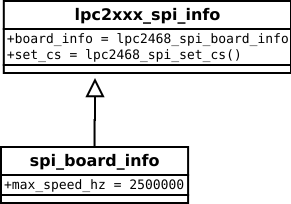
\includegraphics[width=2in]{./uml_logical_spi_lpc24xx}
\caption{UML spi\_info}
\label{fig:uml_logical_spi_lpc24xx}
\end{figure}
The peripherals are initialized in a seperate file called arch/arm/mach-lpc22xx/lpc24xx\_devices.c.
\begin{Verbatim}[fontsize=\footnotesize]
/* -------------------------------------------------------------------- 
* SPI (Chapter 19) * 
-------------------------------------------------------------------- */
/* 
 * lpc2xxx_spi_pdata must be created and initialized in 
 * the board specific file (see e.g. ea_lpc2478_board.c). 
 */ 
extern struct lpc2xxx_spi_info lpc2xxx_spi_pdata;

#if defined(CONFIG_SPI_LPC2XXX) 
static struct resource lpc2xxx_spi_resource[] = {
  { 
    .name = "lpc2xxx-spi", 
    .start = APB_SPI_BASE, 
    .end = APB_SPI_BASE + APB_SPI_SIZE - 1, 
    .flags = IORESOURCE_MEM, 
  }, 
  { 
    .name = "lpc2xxx-spi", 
    .start = LPC2xxx_INTERRUPT_SPI0, 
    .flags = IORESOURCE_IRQ, 
  },
}; 

static struct platform_device lpc2xxx_spi_device = { 
  .name = "lpc2xxx-spi", 
  .id = -1, 
  .num_resources = ARRAY_SIZE(lpc2xxx_spi_resource), 
  .resource = lpc2xxx_spi_resource, 
  .dev = { 
    .platform_data = &lpc2xxx_spi_pdata, 
  }, 
};

static void __init lpc2xxx_add_spi_device(void) { 
  platform_device_register(&lpc2xxx_spi_device); 
} 
#else 
static void __init lpc2xxx_add_spi_device(void) {} 
#endif 
\end{Verbatim}
Also note that some definitions of registers, structures etc are given in \texttt{include/asm/arch-lpc22xx} folder as well. These are not so important as I saw the content. But noteworthy.
\begin{Verbatim}[fontsize=\footnotesize]
board.h        entry-macro.S  irq.h       lpc2xxx_pmc.h  serial.h  uncompress.h
clocks.h       gpio.h         irqs.h      memory.h       system.h
debug-macro.S  hardware.h     keyboard.h  nvram.h        time.h
dma.h          io.h           lpc22xx.h   param.h        timex.h
\end{Verbatim}
Also symlink to this folder is automatically created. So \texttt{linux-2.6.x/include/asm/arch} is symlinked of \texttt{linux-2.6.x/include/asm-arm/arch-lpc22xx}.

\section{DRIVER INITIALIZATION}
The static platform driver structure\texttt{ lp2xx\_spidrv} is initialized with a \texttt{spi\_probe} function. The  driver's name is set to \texttt{lpc2xxx-spi} which matches with the device's name. Because of that when the \\
\texttt{platform\_driver\_register} is called with this driver structure, the binding is done between the driver and device. \texttt{lpc2xxx\_spi\_device} above is defined as the platform device with the same name 
\begin{Verbatim}[fontsize=\footnotesize]
static struct platform_driver lpc2xxx_spidrv = {
	.probe		= lpc2xxx_spi_probe,
....
	.driver		= {
		.name	= "lpc2xxx-spi",
		.owner	= THIS_MODULE,
	},
};

static int __init lpc2xxx_spi_init(void)
{
  return platform_driver_register(&lpc2xxx_spidrv);
}

module_init(lpc2xxx_spi_init);
\end{Verbatim}

spi\_probe starts by pointers to may different structures. Most notably spi\_master and lpc2xxx\_spi. The goal in the init routine is to set these to valid memory locations. The spi device acts as the spi-master. It starts by call to allocate memory for spi master. The size of the private data for the driver is given and the newly allocated memory pointer to a master struct is returned. The private data (lpc2xxx\_spi) pointer is assigned a valid memory by spi\_master\_get\_devdata. The memory is in the class private data. Now the private data has few member that are initialized to master, platform\_data, platform\_device. The private data consists of bitbang structure since lpc2468 supports that as of this writing. Its master, setup\_transfer, chipselect, txrx\_bufs, setup are setup appropriately. A UML diagram is given. A resource object is retrieved from the platform data. Memory, IO Area, and Interrupts are set for the private data. When the memory is requested, it actually creates a busy region with interlocks. Memory is remapped and the IRQ is requested to the kernel. When IRQ is requested, the IRQ line, the handler, etc.. are sent to the kernel. From that point on interrupts can be generated. So a service routine should be able to handle it. IO remap maps arbitrary physical memory to kernel virtual address space so that the kernel can execute code in external memory.  The SPI control register is enabled for master mode and for interrupt generation when transfer is completed. Bitbang driver is started and any further requested are assumed to be handled by the driver. Finally a call is done to add the new spi device giving the master and board information object  

\paragraph{}In short, a spi\_master obj is created. A private object that contains specific information about our driver is initialized. Memory, IRQ, hardware registers are setup. Finally the new device is added as a spi device to kernel core. 

\section{TRANSFER}
SPI communication happens as transfers. Transfers are made up of 8 bit words or other sizes depending on the configuration. LPC24xx is configured to use the bit bang driver. 
\subsection{SETUP}
First the driver is setup to do transfers and then \texttt{spi\_bitbang\_transfer()} function can be called to do the actual transfer. bitbang object is created in the spi\_device private data. It's setup\_transfer function is initialized to \texttt{lpc2xxx\_spi\_setupxfer} which does the real work. A user interacting driver code, such as one that of a SPI based ADC, will call \texttt{spi\_bitbang\_setup()} first which will dereference the function pointer for \texttt{bitbang->setup\_transfer()} The dereference will result in \texttt{lpc2xxx\_spi\_setupxfer} being called. In this function, a prescalar is set up in SPI0 Control register and the chipselect set to be in INACTIVE mode. In LPC24xx the bits per word are 8. 

\begin{table}[ht]
\centering
\resizebox{\textwidth}{!}
{\begin{tabular}{|c|c|c|c|}
\hline Object & Function Ptr  & Value & Call \\ 
\hline spi\_lpc2xxx & setup\_transfer() & lpc2xxx\_spi\_setupxfer() & spi\_bitbang\_setup \\ 
\hline 
\end{tabular}}
\caption{Setup of Function Pointer} 
\end{table}

\subsection{TRANSMIT/RECEIPT}
The actual transfer happens when the spi\_bitbang\_transfer() function is called. It deferences the function pointer txrx\_bufs which results in lpc2xxx\_spi\_txrx being called. Of course txrx\_bufs is initialized by the driver code to lpc2xxx\_spi\_txrx.
Internally spi\_bitbang\_transfer function puts the transfer message in a kernel work queue and a separate function processes the queue. spin\_locks are used during the work queue processing  When the driver transfer function is called, the pointer to transmit buffer, the length of transfer etc are setup and writeb() is called to write the data byte by byte to the SPI0 data register. The routine waits for the completion of the transfer using wait queue. As in the init routine interrupt is generated when a transfer is completed. Upon completion it clears the wait queue so that another transaction can be started. The whole transfer happens till every data is completely transfered. 

\subsubsection{INTERRUPT SERVICE ROUTINE}
The interrupt service routine is registered when a new spi\_device is added as in the probe routine. Its called whenever a tranfer is completed. In it it reads the status register of SPI0, and checks for write collision or spi device not ready for transfer. it then increments the count and if needed reads byte from the data register, Work queue is cleared to start another transaction. <completion.h> describes how to work with wait queues.  

\section{TODO}
a. clock timing for SPI ? How is it architected?\\
b.  
\end{document}